% Asset ID: FA21IntegrationTechniquesTikZ-001
% Unit: FA21 Further A2 1 Pure Mathematics
% Topic code: FA21-FCALC
% Topic ID: FA21IntegrationTechniques
% Related lesson file: FA21_integration_techniques_lesson.md
% Related lesson section: # 9. Visual Asset Integration
% Used placeholder: [VISUAL PLACEHOLDER: FA21IntegrationTechniquesTikZ-001 | Source: Transcript examples for I_4=
% \\int x^4e^x\\,dx, I_5, and I_6 | Insert from tikz/FA21IntegrationTechniquesTikZ-001.tex | Purpose: Provide a precise mathematical recurrence diagram for printed notes.]
% Source: Teacher transcript examples for I_4 = integral x^4 e^x dx and recurrence substitution.
% Purpose: Provide a precise recurrence diagram showing I_4 -> I_3 -> I_2 -> I_1 -> I_0, with arrows showing substitution upwards into I_4.

\documentclass[tikz,border=8pt]{standalone}
\usepackage{amsmath}
\usepackage{xcolor}
\usetikzlibrary{arrows.meta, positioning, calc, backgrounds}
\definecolor{Canvas}{HTML}{FAF9F6}
\definecolor{Ivory}{HTML}{FFFFF0}
\definecolor{LineGrey}{HTML}{E5E5EA}
\definecolor{Gold}{HTML}{C5A059}
\definecolor{SoftGold}{HTML}{D4AF37}
\definecolor{Blush}{HTML}{FBEFEF}
\definecolor{TextInk}{HTML}{2C2C2E}
\begin{document}
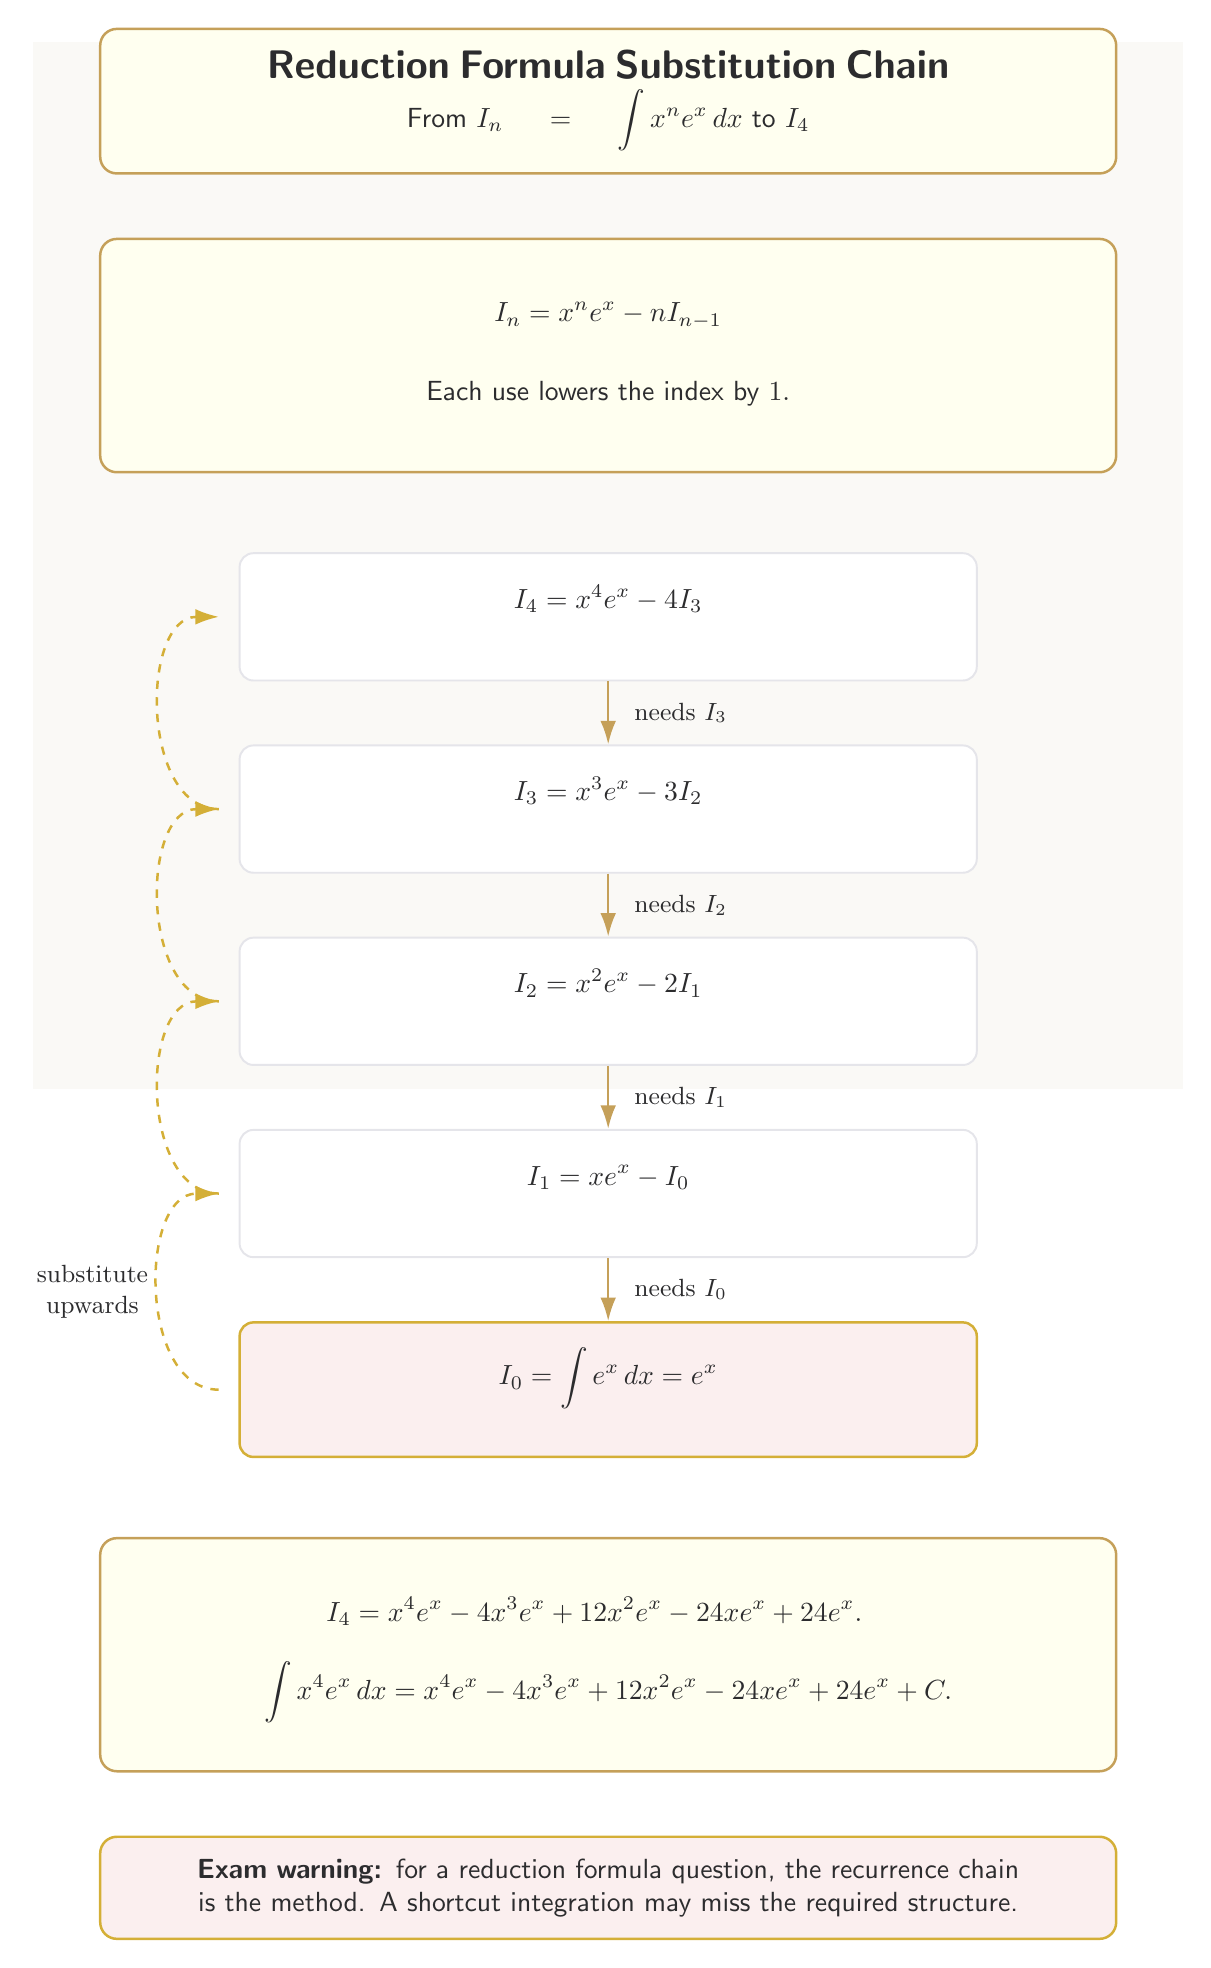
\begin{tikzpicture}[font=\sffamily,every node/.style={text=TextInk},recurrencebox/.style={draw=LineGrey,fill=white,rounded corners=5pt,line width=0.7pt,inner xsep=8pt,inner ysep=8pt,text width=8.8cm,align=left},basebox/.style={draw=SoftGold,fill=Blush,rounded corners=5pt,line width=0.9pt,inner xsep=8pt,inner ysep=8pt,text width=8.8cm,align=left},titlebox/.style={draw=Gold,fill=Ivory,rounded corners=6pt,line width=0.9pt,inner xsep=10pt,inner ysep=8pt,text width=12.2cm,align=center},goldarrow/.style={-{Latex[length=3mm,width=2mm]},draw=Gold,line width=0.9pt},backarrow/.style={-{Latex[length=3mm,width=2mm]},draw=SoftGold,line width=0.9pt,dashed}]
\begin{scope}[on background layer]\fill[Canvas] (-7.3,-11.2) rectangle (7.3,2.1);\end{scope}
\node[titlebox] (title) at (0,1.35) {{\Large\bfseries Reduction Formula Substitution Chain}\\[3pt] From \(\displaystyle I_n=\int x^n e^x\,dx\) to \(\displaystyle I_4\)};
\node[titlebox, below=8mm of title] (formula) {\[I_n=x^n e^x-nI_{n-1}\]\vspace{-2mm}\[\text{Each use lowers the index by }1.\]};
\node[recurrencebox, below=10mm of formula] (I4) {\[I_4=x^4e^x-4I_3\]};
\node[recurrencebox, below=8mm of I4] (I3) {\[I_3=x^3e^x-3I_2\]};
\node[recurrencebox, below=8mm of I3] (I2) {\[I_2=x^2e^x-2I_1\]};
\node[recurrencebox, below=8mm of I2] (I1) {\[I_1=xe^x-I_0\]};
\node[basebox, below=8mm of I1] (I0) {\[I_0=\int e^x\,dx=e^x\]};
\draw[goldarrow] (I4.south) -- node[right,xshift=2mm,font=\small] {needs \(I_3\)} (I3.north);
\draw[goldarrow] (I3.south) -- node[right,xshift=2mm,font=\small] {needs \(I_2\)} (I2.north);
\draw[goldarrow] (I2.south) -- node[right,xshift=2mm,font=\small] {needs \(I_1\)} (I1.north);
\draw[goldarrow] (I1.south) -- node[right,xshift=2mm,font=\small] {needs \(I_0\)} (I0.north);
\draw[backarrow] ($(I0.west)+(-0.25,0)$) to[out=180,in=180,looseness=1.05] node[left,font=\small,align=center] {substitute\\upwards} ($(I1.west)+(-0.25,0)$);
\draw[backarrow] ($(I1.west)+(-0.25,0)$) to[out=180,in=180,looseness=1.05] ($(I2.west)+(-0.25,0)$);
\draw[backarrow] ($(I2.west)+(-0.25,0)$) to[out=180,in=180,looseness=1.05] ($(I3.west)+(-0.25,0)$);
\draw[backarrow] ($(I3.west)+(-0.25,0)$) to[out=180,in=180,looseness=1.05] ($(I4.west)+(-0.25,0)$);
\node[titlebox, below=10mm of I0] (answer) {\[\begin{aligned}I_4&=x^4e^x-4x^3e^x+12x^2e^x-24xe^x+24e^x.\end{aligned}\]\[\int x^4e^x\,dx=x^4e^x-4x^3e^x+12x^2e^x-24xe^x+24e^x+C.\]};
\node[draw=SoftGold,fill=Blush,rounded corners=6pt,line width=0.9pt,inner xsep=10pt,inner ysep=8pt,text width=12.2cm,align=center,below=8mm of answer] {\textbf{Exam warning:} for a reduction formula question, the recurrence chain is the method. A shortcut integration may miss the required structure.};
\end{tikzpicture}
\end{document}
